\documentclass[a4paper,conference]{IEEEtran}
\usepackage{cite}
\usepackage{graphicx}
\usepackage{booktabs}
\usepackage{balance}
\graphicspath{{../figures/isainlp2026/}}

\begin{document}

\title{Diagnosing Candidate Exposure after Held-Out Confirmation in Cross-Domain Patent Retrieval}
\author{Anonymous Author(s)}
\maketitle

\begin{abstract}
A retrieval score does not reveal whether relevant patent families were ordered
too low or never entered the candidate pool. We study this distinction after
model selection, using one frozen dense retriever on the domain-aware DAPFAM
benchmark. The system first improved Recall@100 over BM25 by 0.111379 on 872
held-out out-of-domain queries (95\% paired-bootstrap confidence interval
[0.102294, 0.120438]). We then materialized the unchanged system over 45,336
documents and 1,247 queries and audited its family Top-200 pool without
reopening selection. No relevant family appeared in the pool for 455 of 905
out-of-domain queries; across 5,193 relevant-family incidences, 4,065 were
absent at rank 200. Perfect ordering of candidates already in the pool could
raise macro Recall@100 only from 0.188450 to 0.260167, an analytical upper
bound of 0.071717. Query classes, incidence counts, and macro Recall use
different aggregation rules and are not additive. This receipt-bound,
single-system DAPFAM case study shows how a frozen-pool audit can separate
candidate availability from ordering headroom while preserving the boundary
between confirmation and diagnosis.
\end{abstract}

\begin{IEEEkeywords}
patent retrieval, domain shift, candidate generation, diagnostic evaluation,
reproducibility
\end{IEEEkeywords}

\section{Introduction}
Patent search must retrieve technically related documents despite differences
in terminology, drafting practice, and technology domain. Family-level
benchmarks expose this difficulty by grouping related filings and evaluating
whether a retrieval system finds the relevant families. DAPFAM makes the domain
boundary explicit and reports a marked gap between in-domain and out-of-domain
retrieval~\cite{ayaou2025dapfam}. A recent evaluation of patent embeddings also
finds that model quality varies by task and domain~\cite{yousefiramandi2026patent}.

Recall at a declared depth is essential, but it compresses two operationally
different failures. A relevant family may be in the candidate pool but ranked
below the evaluation cutoff, or it may be absent from the pool. A reranker can
address the first case only for candidates it receives~\cite{nogueira2019passage}.
This boundary is familiar in multi-stage retrieval, yet it is easy to obscure
when a final score is reported without a depth audit. The problem is sharper
under domain shift, where poor lexical or semantic matching may prevent
relevant material from being exposed at all.

We ask: \emph{after a retrieval configuration has been confirmed and frozen,
how much of its out-of-domain shortfall is visible as candidate absence, and
how much macro-Recall headroom remains through ordering within the observed
pool?} We answer with an audited measurement study, not a new metric or
reranking method. One dense configuration was selected before the analysis and
compared once with BM25 on 872 held-out out-of-domain queries. The unchanged
configuration was then run over the complete benchmark, and its deterministic
family Top-200 pool was diagnosed without another selection or final access.

The central finding appears at two counting levels. No relevant family reached
the Top-200 pool for 455 of 905 out-of-domain queries. Across all 5,193
out-of-domain relevant-family incidences, 4,065 were absent at rank 200. An
oracle ordering of the same pool raised macro Recall@100 from 0.188450 to
0.260167, leaving 0.071717 ordering headroom. The query classes, incidence
counts, and macro average have different units; none decomposes another.

The empirical contribution is a receipt-bound, two-level exposure audit of one
selected DAPFAM retriever. It connects held-out confirmation to complete-corpus
diagnosis and shows that the incidence deficit spans 455 of 905 OUT queries.
The fixed-pool oracle then bounds what ordering alone could recover without
presenting a reranker result.

\begin{figure*}[t]
\centering
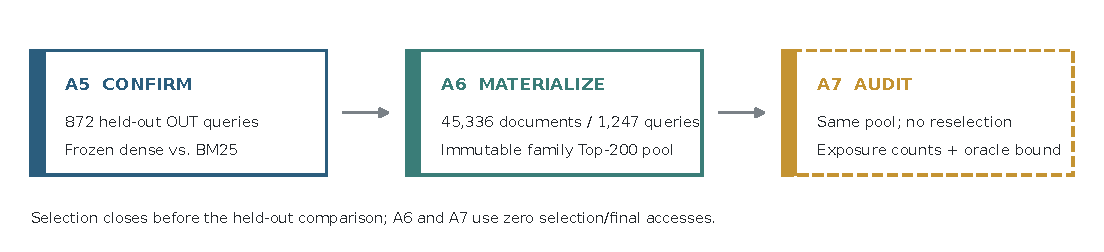
\includegraphics[width=\textwidth]{evidence_chain.pdf}
\caption{Evidence sequence and freeze boundary. A5 is the single held-out
comparison. A6 materializes the frozen winner over the complete benchmark.
A7 audits that same pool: exposure states are measured counts, whereas the
fixed-pool oracle is an analytical upper bound. Neither A6 nor A7 reopens model
selection or accesses the held-out final set.}
\label{fig:evidence}
\end{figure*}

\section{Related Work}
\subsection{Patent Retrieval under Domain Shift}
DAPFAM evaluates prior-art retrieval at the patent-family level and defines
domain-aware benchmark strata~\cite{ayaou2025dapfam}. Its family-level relevance
structure avoids counting multiple filings of the same invention as independent
targets. Broader patent-embedding evidence shows that no single model ordering
holds across retrieval, classification, clustering, and domain
conditions~\cite{yousefiramandi2026patent}. These studies motivate explicit
domain reporting. Our study uses DAPFAM as an existing benchmark and does not
claim a new dataset or an external comparison with results produced under
unverified protocols.

\subsection{Candidate Generation and Ordering}
BM25 remains a standard lexical reference~\cite{robertson2009probabilistic},
while dense retrieval supports semantic matching at large scale
~\cite{karpukhin2020dense}. Heterogeneous benchmarks such as BEIR evaluate
first-stage retrieval across tasks~\cite{thakur2021beir}. Late-interaction and
approximate-nearest-neighbor systems make the candidate-depth tradeoff explicit
~\cite{khattab2020colbert,xiong2021ance}. Reranking work, in turn, evaluates
reordering within a retrieved set~\cite{nogueira2019passage}. These lines of
work establish that downstream ordering is bounded by candidate generation.
Our narrower contribution is to measure that boundary on one immutable,
post-confirmatory family pool and to keep incidence counts distinct from a
macro-Recall oracle.

\section{Study Design}
\subsection{Benchmark and Evidence Boundary}
DAPFAM contains 1,247 evaluated queries and 45,336 source documents in the
complete materialization used here. The receipt-defined in-domain and
out-of-domain strata contain 1,217 and 905 judged queries. These stratum counts
are not additive; all aggregate metrics retain the evaluator's declared query
population. Family relevance is binary. We report macro Recall and nDCG at the
declared cutoff using their standard definitions~\cite{jarvelin2002cumulated}.

The analysis begins after development selection. Earlier screening and system
search produced one frozen dense configuration, but their exploratory values
are outside this paper's quantitative argument. Figure~\ref{fig:evidence}
shows the retained evidence sequence. A5 used one held-out final access to
compare the frozen configuration with a static BM25 reference. A6 applied the
winner to the complete corpus and wrote a deterministic family Top-200 pool.
A7 read that pool on CPU and produced aggregate-safe diagnostics. Integrity
audits record zero selection and final accesses for A6 and A7, no winner change,
no pool expansion, and no protected rankings in the public outputs.

Before confirmation, A4 froze a registry of four finalists. One Selection-125
access covered all 125 queries; the declared OUT metric denominator was 90.
Six preregistered pairwise comparisons used 10,000 bootstrap resamples and
Holm--Bonferroni correction. The predeclared selection rule prioritized OUT
Recall@100, then nDCG@100 for Recall differences below 0.005, and then nDCG@10
for nDCG@100 differences below 0.002. Remaining ties used latency, cost and
index size, and finally configuration simplicity. A4 used zero final accesses.
Selection-125 and Final-872 were separate frozen scopes governed by the same
parent split commitment; no membership or protected identifier is disclosed.

\subsection{Frozen Retrieval Configuration}
We use the PatEmbed-large checkpoint from datalyes and a \texttt{bm25s}
reference over the same title, abstract, and claims fields. The dense
representation uses 384-token passages with 64-token overlap, normalized-vector
search, and maximum-score aggregation at the patent-family level.

Model, representation, chunking, retrieval, index, and runtime configurations
were hash-bound before complete-corpus materialization. A6 covered all 45,336
documents and all 1,247 queries without failure, yielding exactly 249,400 rows
in the family Top-200 pool. SHA-256 prefixes bind the A5 winner configuration
(\texttt{285e94b1e76b}), A6 model manifest (\texttt{0ae9ed779d0e}), and A6
execution configuration (\texttt{e560e565e451}); the release manifest records
the full digests. The public package excludes query identifiers, family
membership, relevance judgments, rankings, and per-query outcomes.

\subsection{Held-Out Confirmation}
The confirmatory comparison contains 872 held-out out-of-domain queries and two
frozen systems. Each query is the pairing unit. Percentile confidence intervals
use 10,000 nonparametric bootstrap resamples from the frozen evaluation stream
~\cite{davison1997bootstrap}. The final set was accessed once, both systems
completed all 872 queries, and the winner was fixed before the complete-corpus
run. This comparison supports a benchmark- and split-specific effect; it does
not establish universal superiority.

\subsection{Fixed-Pool Diagnosis}
\begin{figure*}[!t]
\centering
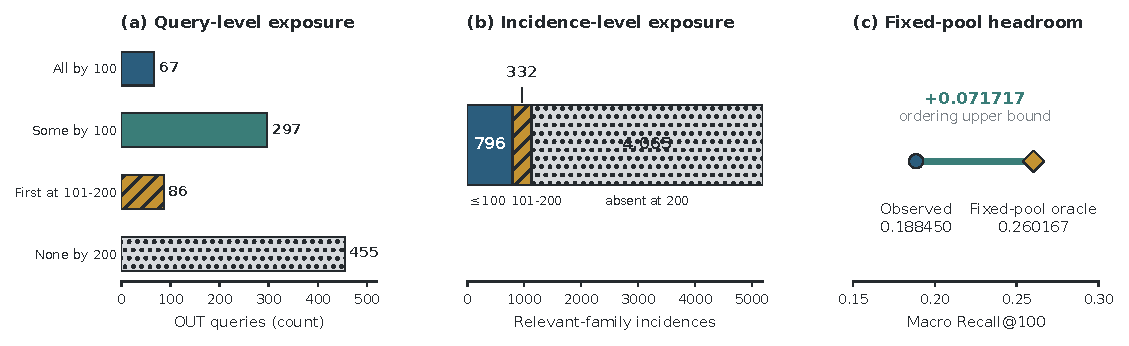
\includegraphics[width=\textwidth]{out_domain_diagnosis.pdf}
\caption{Three non-additive views of the frozen OUT family Top-200 pool. (a)
The four mutually exclusive query classes sum to 905; ``None by 200'' means no
relevant family is present for that query. (b) Raw relevant-family incidence
counts sum to 5,193. (c) Macro Recall@100 is averaged over the 905 queries; the
oracle reorders only candidates already present at rank 200. Query counts,
incidence counts, and macro Recall have different units.}
\label{fig:diagnosis}
\end{figure*}

For every relevant-family incidence in the frozen pool, A7 records one of three
mutually exclusive states: exposed by rank 100, first exposed at ranks
101--200, or absent at rank 200. These are raw counts of query--relevant-family
incidences. They are useful for describing pool composition but are not
components of macro Recall because queries have different relevance-set sizes.

A separate query-level classification records whether all relevant families
were exposed by rank 100, some were exposed by rank 100, the first appeared at
ranks 101--200, or none appeared by rank 200. These four classes are mutually
exclusive and cover the 905 OUT queries. The last class means that no method
restricted to that query's Top-200 pool can retrieve a relevant family.

The ordering diagnostic replaces the observed order within each Top-200 family
pool with an oracle order that places all already retrieved relevant families
first. Ordering headroom is the oracle macro Recall@100 minus observed macro
Recall@100 on the same query population. The oracle cannot introduce a family
that is absent at rank 200. It is therefore an analytical upper bound on
reordering within this pool, not the performance of a learned reranker.

As a descriptive integrity sensitivity, A7 also removed 40 raw self-relations.
OUT Recall@100 and nDCG@100 remained exactly 0.188450 and 0.070644. This check
does not inspect protected split membership and is not a broader leakage audit.

\section{Results}
\subsection{The Frozen System Confirms on Held-Out Queries}
Table~\ref{tab:confirm} reports the single held-out comparison. The dense system
reached Recall@100 of 0.442476, compared with 0.331097 for BM25. The paired
difference was +0.111379, with a 95\% confidence interval of [0.102294,
0.120438]. The nDCG@100 difference was +0.086342, with interval [0.078673,
0.094077]. These results justify carrying the frozen dense configuration into
the post-confirmatory materialization; they do not compare all systems at full
benchmark scale.

\begin{table}[t]
\centering
\caption{Held-out Final-872 OUT comparison. Values are macro means; $\Delta$
is dense minus BM25. The paired 95\% bootstrap intervals are [0.102294,
0.120438] for Recall and [0.078673, 0.094077] for nDCG. Higher is better.}
\label{tab:confirm}
\footnotesize
\begin{tabular}{@{}lrrr@{}}
\toprule
Metric & Dense & BM25 & $\Delta$ \\
\midrule
Recall@100 & 0.442476 & 0.331097 & +0.111379 \\
nDCG@100   & 0.365595 & 0.279253 & +0.086342 \\
\bottomrule
\end{tabular}
\end{table}

\subsection{Complete-Scale Retrieval Retains a Domain Gap}
The unchanged configuration processed all 45,336 source documents and produced
the complete 1,247-query family Top-200 pool. Aggregate Recall@100 was 0.438965
and nDCG@100 was 0.362497. Recall@100 was 0.528164 on the receipt-defined
in-domain stratum and 0.188450 on the out-of-domain stratum; the corresponding
nDCG@100 values were 0.406513 and 0.070644. This is a within-system domain
diagnosis at complete scale, not a full-scale superiority claim against BM25 or
another dense model.

\subsection{Candidate Absence Appears at Query and Incidence Levels}
Figure~\ref{fig:diagnosis} first classifies the 905 out-of-domain queries. All
relevant families were exposed by rank 100 for 67 queries, and some were
exposed for 297. Another 86 had their first relevant family at ranks 101--200.
The remaining 455 had no relevant family in Top-200. Candidate absence is
therefore not confined to a small subset of queries.

At the incidence level, 796 of 5,193 relevant-family incidences were exposed by
rank 100 and 332 first appeared at ranks 101--200. The remaining 4,065 were
absent at rank 200. Most raw out-of-domain relevance incidences were therefore
unavailable to any method restricted to this candidate pool.

The macro-Recall view answers a different question. Observed out-of-domain
Recall@100 was 0.188450. Perfectly ordering every relevant family already in the
Top-200 pool would raise it to 0.260167, leaving 0.071717 headroom within the
observed pool. This bound does not estimate what a practical reranker would
achieve, nor does it test candidate expansion. It only limits the improvement
available from ordering the fixed candidates.

\section{Discussion}
The held-out result and the fixed-pool diagnosis answer different parts of the
evaluation story. The A5 comparison shows that the selected dense configuration
improved over BM25 on the declared held-out out-of-domain set. It does not show
why complete-scale out-of-domain Recall remains low. The post-confirmatory audit
locates the same candidate boundary at query and incidence levels, then measures
ordering headroom in macro-Recall units, without changing the selected system.

This distinction matters when interpreting a proposed retrieval improvement.
A reranking study can be evaluated against the 0.071717 fixed-pool upper bound,
provided that it uses the same pool and population. A candidate-generation
study instead needs to test whether additional relevant families enter the
pool. The present evidence does not establish either intervention's efficacy.
It identifies which outcome each future study would need to change and prevents
a gain in one quantity from being described as if it explained the other.

Within this single-system DAPFAM case study, the audit also illustrates a
governance benefit. Model selection, held-out
confirmation, complete-corpus execution, and post-confirmatory diagnosis are
separated by frozen hashes and access counters. This separation does not make
the experiment independently rerunnable without protected benchmark inputs,
but it makes the claim boundary inspectable: the diagnostic cannot silently
become another model-selection step.

\subsection{Limitations}
The evidence is limited to DAPFAM, its receipt-defined strata, and one frozen
dense configuration. Full-scale materialization does not compare the screened
systems or BM25, so the held-out system difference must not be projected onto
the complete-corpus result. The IN and OUT strata are benchmark-defined and
their query counts are not additive. The incidence analysis is descriptive;
it does not attribute absence to a specific representation mechanism.

The oracle assumes perfect ordering of known relevant families already present
in each Top-200 pool. It is not a reranker evaluation, and no pool-expansion
experiment was performed. External protocol settings were not verified well
enough for a cross-paper performance comparison. Protected query identifiers,
rankings, relevance judgments, and per-query outcomes are withheld, so the
public artifact supports aggregate claim auditing rather than independent
end-to-end reproduction. No causal, legal, or external-generalization claim
follows from these results.

\balance
\section{Conclusion}
One held-out score cannot show where cross-domain retrieval fails. In this
receipt-bound case study of one DAPFAM system, a frozen dense patent retriever
improved over BM25 on 872 held-out queries. Yet 455 of 905 complete-scale OUT
queries had no relevant family in Top-200, and 4,065 of 5,193 relevant-family
incidences were absent. Within that same pool, perfect ordering could raise
macro Recall@100 only from 0.188450 to 0.260167. Keeping the query classes,
incidence counts, and macro bound separate identifies candidate expansion as a
distinct research target while leaving its efficacy, and that of reranking, as
open questions.

\bibliographystyle{IEEEtran}
\bibliography{../references/references}
\end{document}
